\chapter{Testing to inform evaluation}
\section{Testing methods}
In order to carry out testing to inform my project evaluation, I will use both alpha and beta testing methods (GeeksforGeeks, 2022). Alpha testing is a full workings test of the program utilising boundary and erroneous tests alongside the typical program functionality tests. The aim of alpha testing is to eliminate the bugs and check that each function works as it should. The alpha testing will be carried out by me as the developer. By comparison, beta testing will be carried out by the two stakeholders as listed in the analysis section of this report. It aims to test the program in the real-world application the project was designed for. This will mean the stakeholders will walk through and test whether they can login, create listings, bid on listings and other regular functions of the website. Beta testing will ensure that there are no major regular running areas before the project is launched.

\section{Alpha testing}
\begin{center}
\begin{longtable}{|P{23mm}|P{20mm}|P{19mm}|P{20mm}|P{54mm}|}
  \hline
  \textbf{Test} & \textbf{Type} & \textbf{Expected result} & \textbf{Actual result} & \textbf{Test evidence} \\
  \hline
  \endfirsthead
  \hline
  \endhead
  \hline 

  \endfoot
  \endlastfoot

Registration page displays register form & Normal & Form is displayed &
Pass -- as expected &
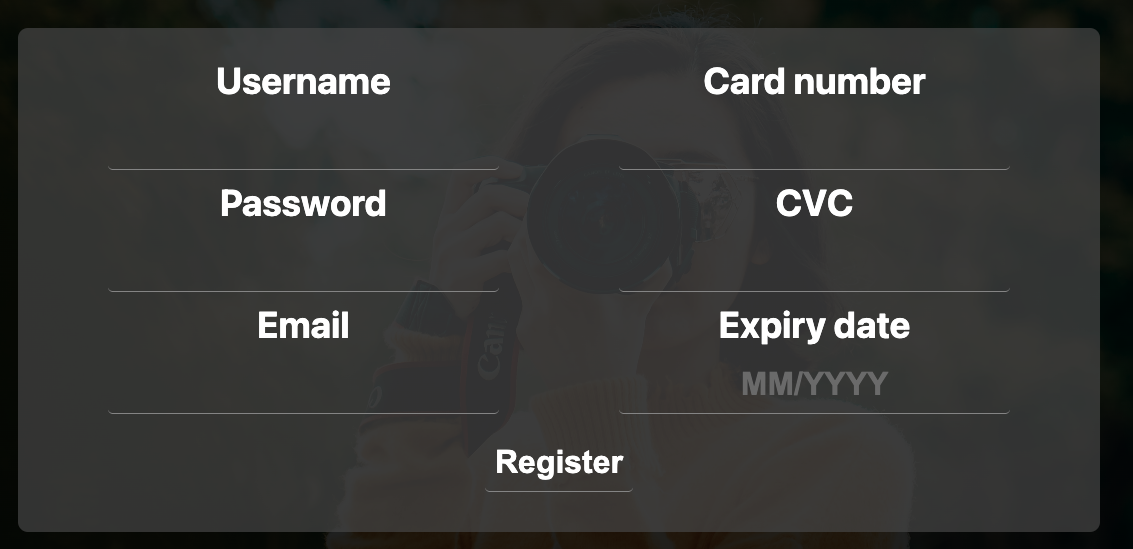
\includegraphics[width=51mm]{ch4_testing_for_eval/media/image2.png} \\ \hline
Form is blank & Erroneous & Error message displayed & Pass -- as
expected &

\includegraphics[width=51mm]{ch4_testing_for_eval/media/image3.png} \\ \hline
Card number or cvc is not text & Erroneous & Form only allows number
input & Pass -- as expected &

\includegraphics[width=51mm]{ch4_testing_for_eval/media/image4.png} \\ \hline
Card number not long enough & Erroneous & Error message to user & Pass
-- as expected &

\includegraphics[width=51mm]{ch4_testing_for_eval/media/image5.png} \\ \hline
CVC not long enough & Erroneous & Error message displayed & Pass -- as
expected &

\includegraphics[width=51mm]{ch4_testing_for_eval/media/image5.png} \\ \hline
Details entered correctly & Normal & Details to database and user
forwarded to home page & Pass -- forwarded to home page &
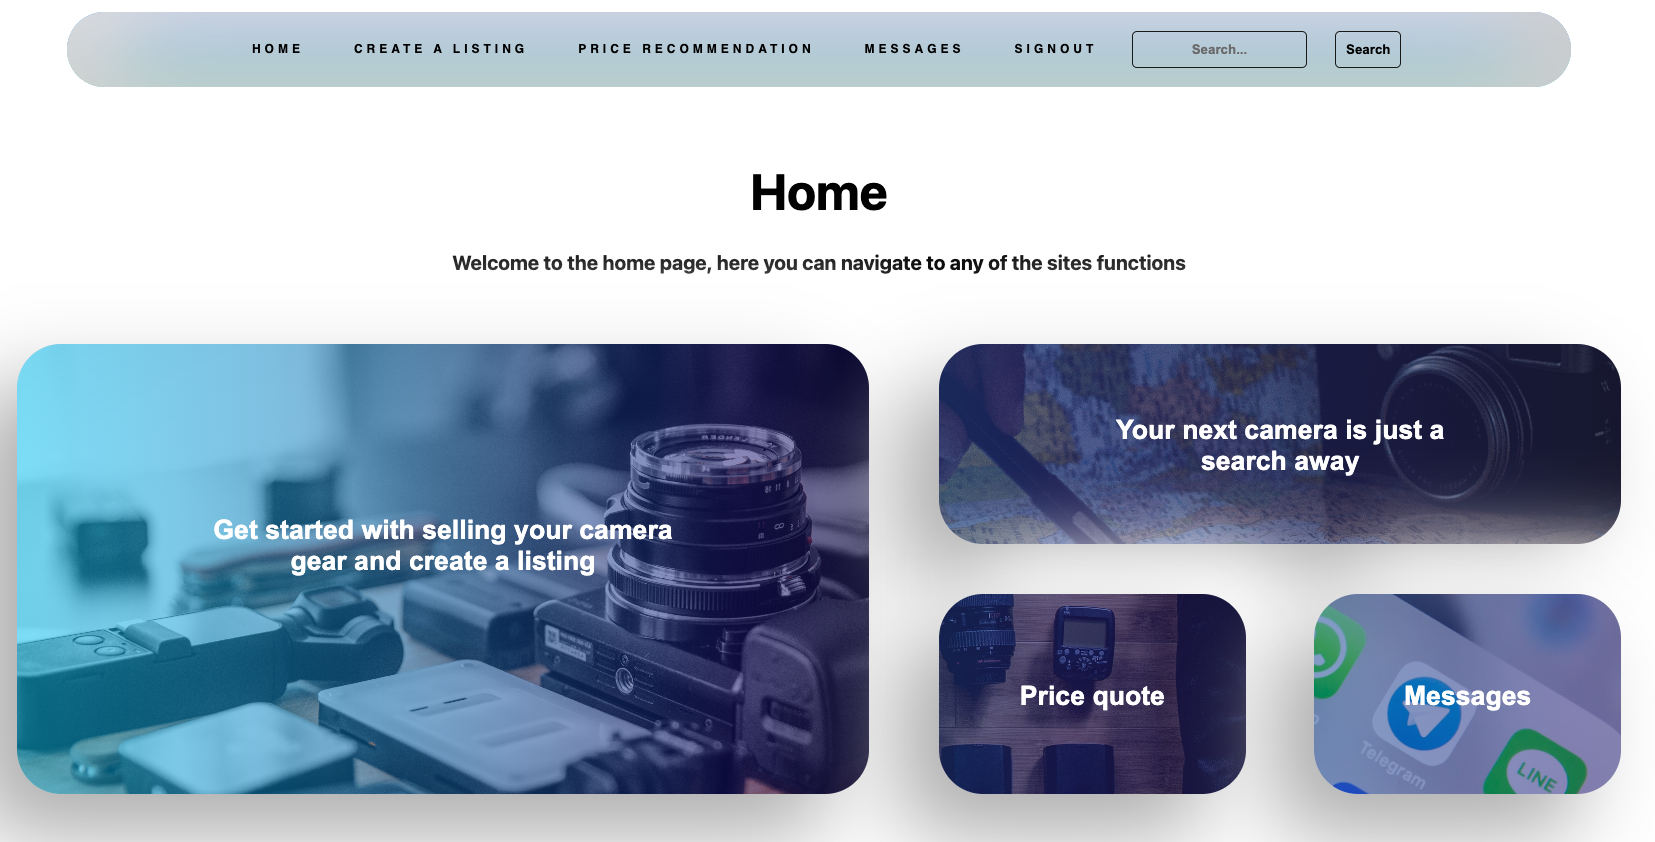
\includegraphics[width=51mm]{ch4_testing_for_eval/media/image6.png} \\ \hline
Registration details are hashed & Normal & Details in database are
hashed & Pass -- all inputs are hashed &
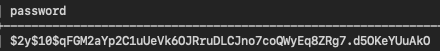
\includegraphics[width=51mm]{ch4_testing_for_eval/media/image7.png}

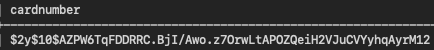
\includegraphics[width=51mm]{ch4_testing_for_eval/media/image8.png}

All are hashed with two columns shown \\
Login page displays form & Normal & Form is displayed to user & Pass --
form is shown &
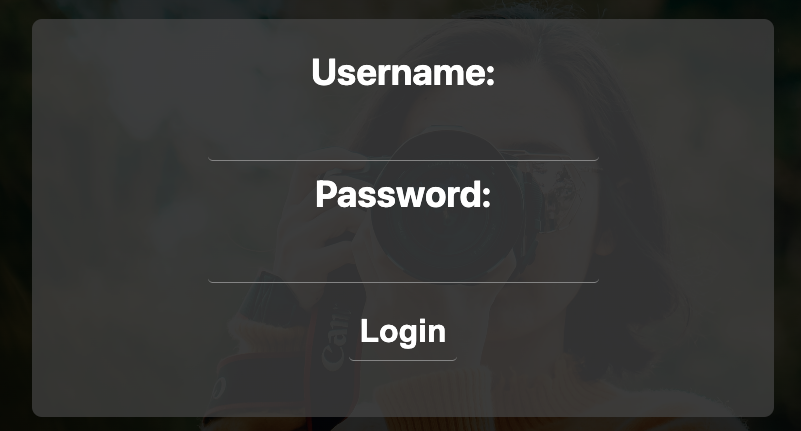
\includegraphics[width=51mm]{ch4_testing_for_eval/media/image9.png} \\ \hline
Login form is submitted blank & Erroneous & Error message shown to user
& Pass -- message shown &

\includegraphics[width=51mm]{ch4_testing_for_eval/media/image10.png} \\ \hline
Login page contains forgot password button & Normal & Button is shown &
Pass -- button appears &

\includegraphics[width=51mm]{ch4_testing_for_eval/media/image11.png} \\ \hline
User is shown form to enter username and email & Normal & The user has a
2-text box form displayed & Fail &
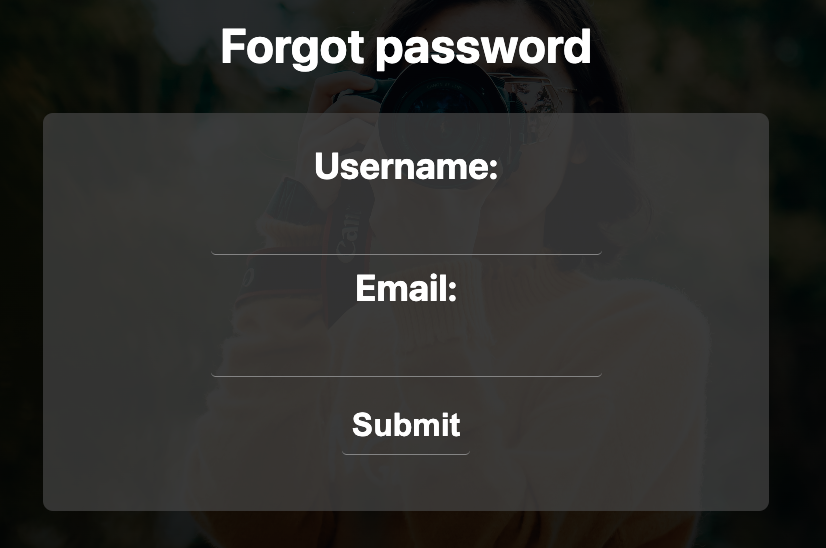
\includegraphics[width=51mm]{ch4_testing_for_eval/media/image12.png} \\ \hline
If username and password match user is sent & Normal & The user is sent
an email with a replacement password & Pass -- email is sent to the user
&
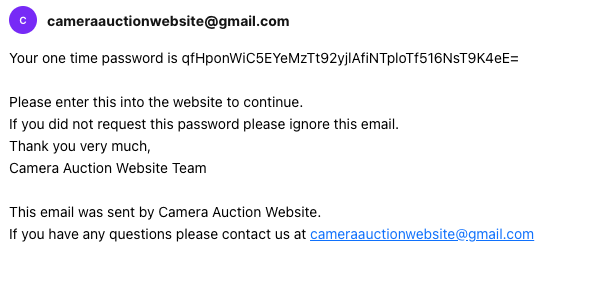
\includegraphics[width=51mm]{ch4_testing_for_eval/media/image13.png} \\ \hline
User is given an error is they do not match & Erroneous & The user is
shown an error & Pass -- message shown &

\includegraphics[width=51mm]{ch4_testing_for_eval/media/image14.png} \\ \hline
User is shown an error if the forms are blank & Erroneous & The user is
shown an error & Pass -- message shown &

\includegraphics[width=51mm]{ch4_testing_for_eval/media/image15.png} \\ \hline
Correct details forwards user to home page & Normal & User is forwarded
to the homepage & Pass -- home page displayed &
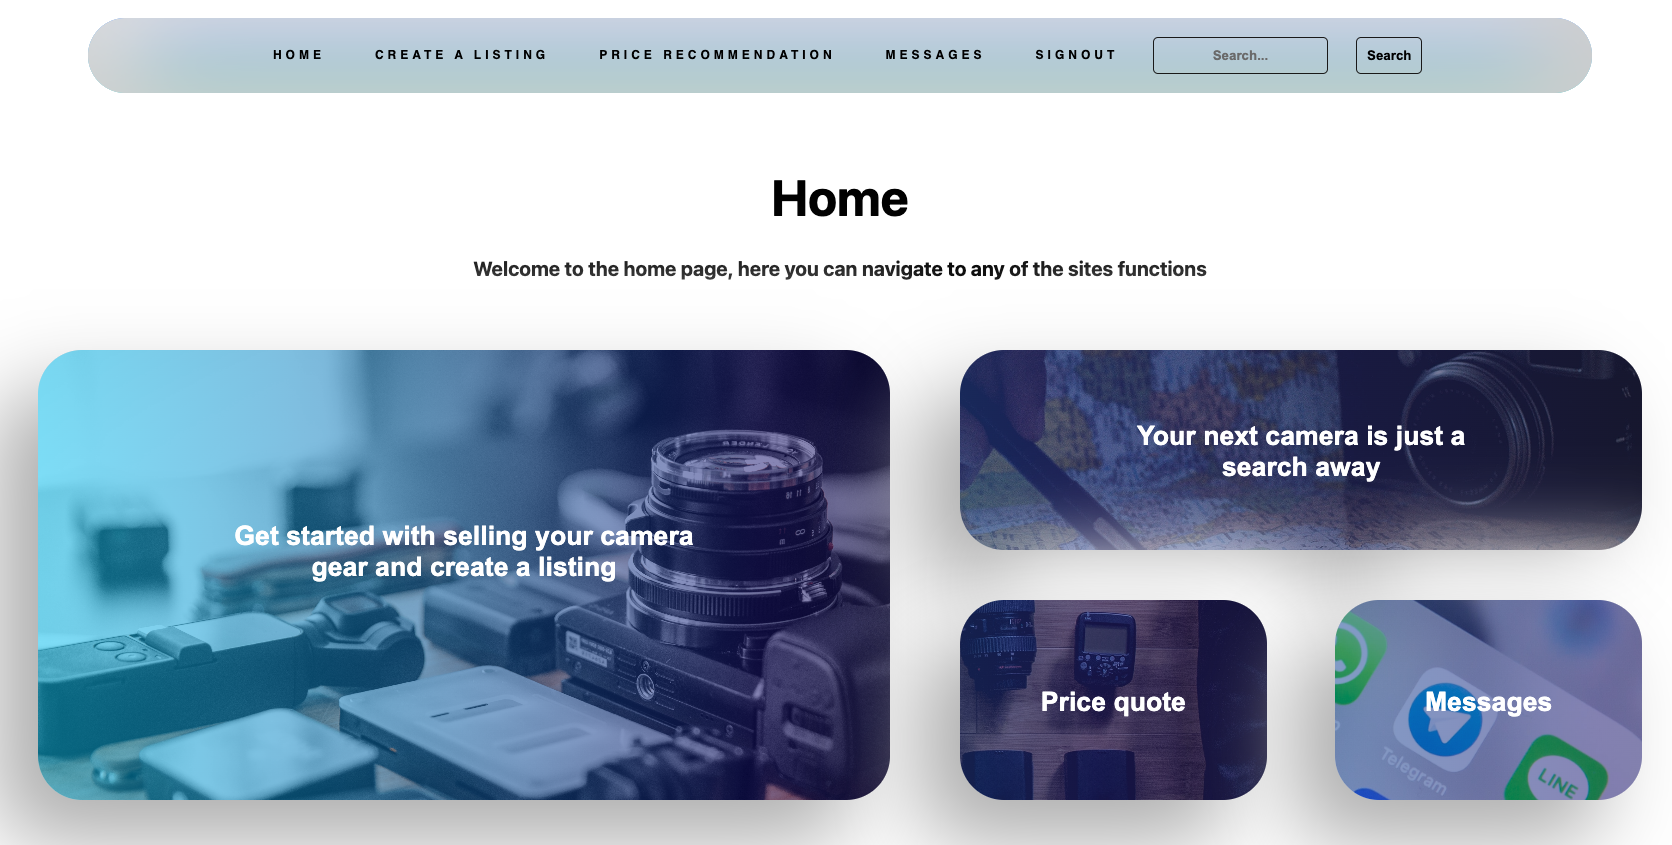
\includegraphics[width=51mm]{ch4_testing_for_eval/media/image16.png} \\ \hline
User enters incorrect details & Erroneous & Details incorrect message &
Pass -- as expected &

\includegraphics[width=51mm]{ch4_testing_for_eval/media/image17.png} \\ \hline
Home page displays navigation bar & Normal & Bar displayed at top of
screen & Pass -- as expected &
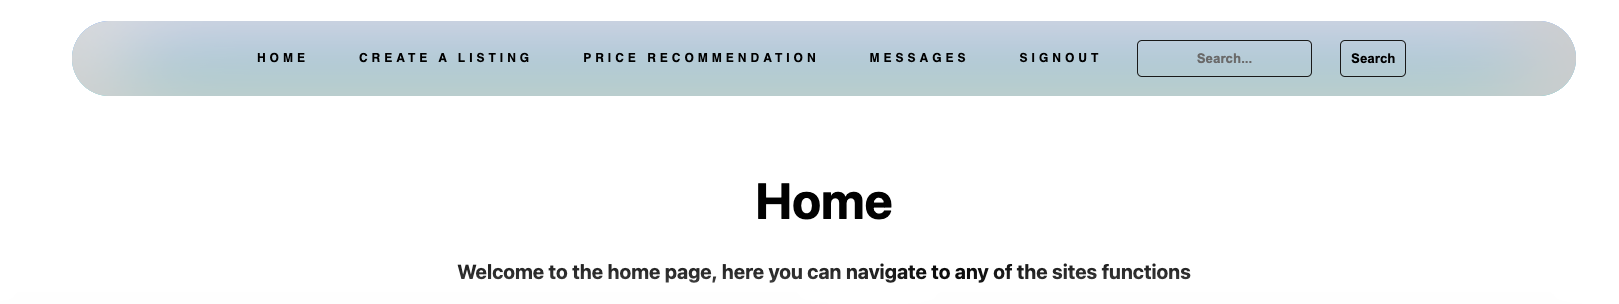
\includegraphics[width=51mm]{ch4_testing_for_eval/media/image18.png} \\ \hline
Home page displays 4 buttons for each page & Normal & Buttons on
homepage with image & Pass -- as expected &

\includegraphics[width=51mm]{ch4_testing_for_eval/media/image19.png} \\ \hline
Create a listing page displays form & Normal & Form shown to user & Pass
-- form is displayed &
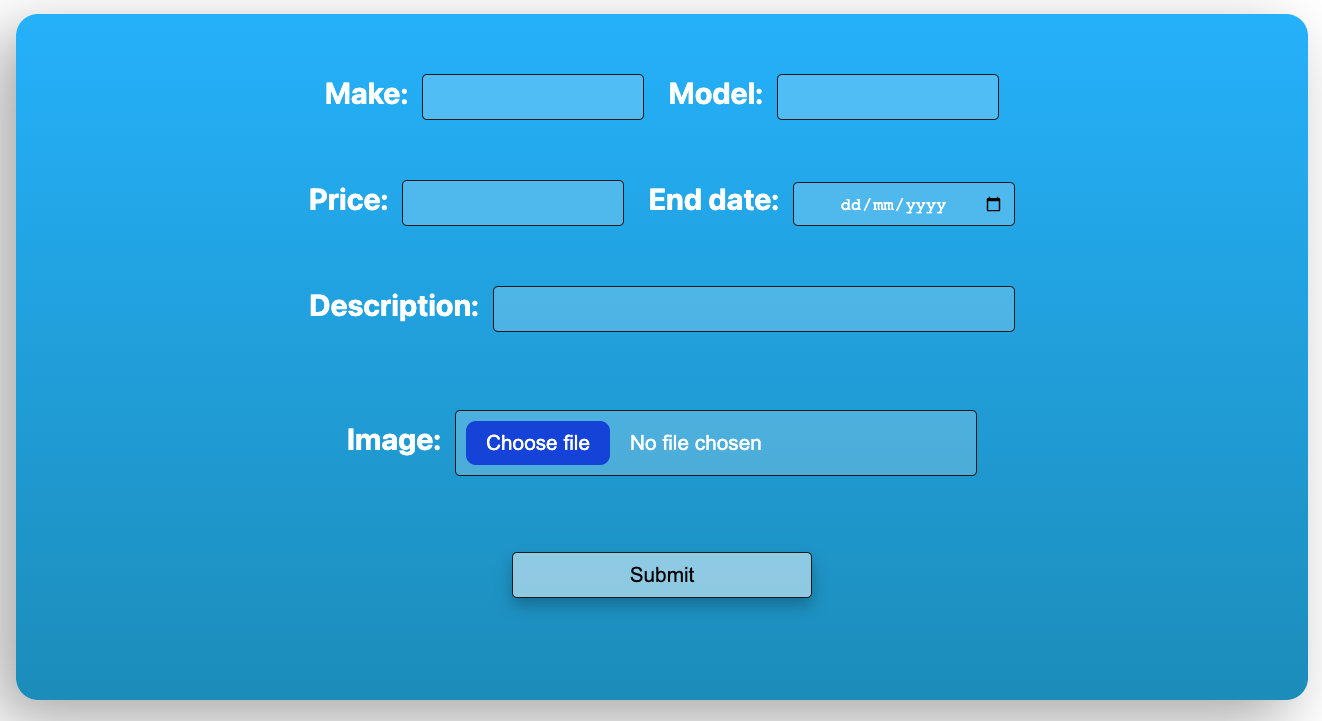
\includegraphics[width=51mm]{ch4_testing_for_eval/media/image20.png} \\ \hline
Create a listing form allows text entry & Normal & User can input text
and file & Pass -- as expected &
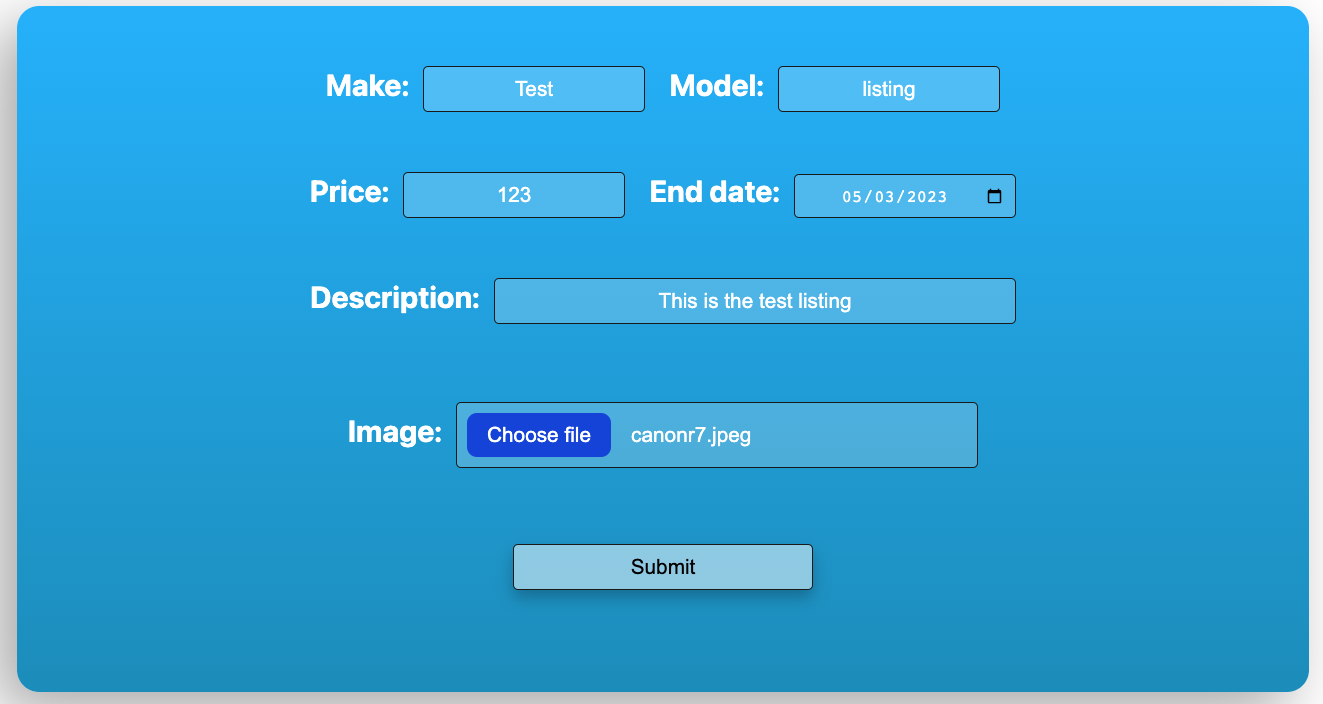
\includegraphics[width=51mm]{ch4_testing_for_eval/media/image21.png} \\ \hline
Submitting a normal listing & Normal & Listing is sent to database &
Pass -- as expected &

\includegraphics[width=51mm]{ch4_testing_for_eval/media/image22.png}

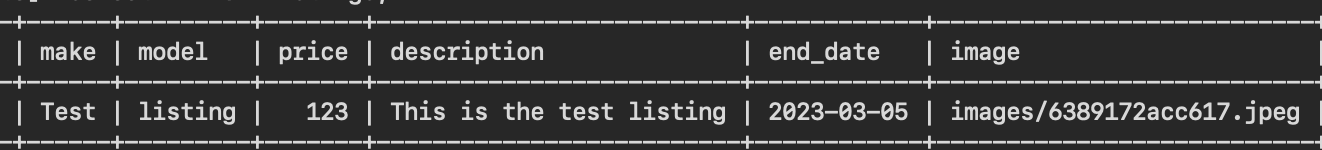
\includegraphics[width=51mm]{ch4_testing_for_eval/media/image23.png} \\ \hline
Listing price is not a number & Boundary & Error message displayed &
Pass -- as expected &

\includegraphics[width=51mm]{ch4_testing_for_eval/media/image24.png} \\ \hline
Create listing form is submitted blank & Boundary & Error message shown
& Pass- as expected &

\includegraphics[width=51mm]{ch4_testing_for_eval/media/image25.png} \\ \hline
Attempt to upload non-image file & Boundary & Not accepted file type
error & Pass -- message shown &

\includegraphics[width=51mm]{ch4_testing_for_eval/media/image26.png} \\ \hline
Navigation search bar searches listings & Normal & Search page with
search term loaded & Pass -- as expected &

\includegraphics[width=51mm]{ch4_testing_for_eval/media/image27.png}

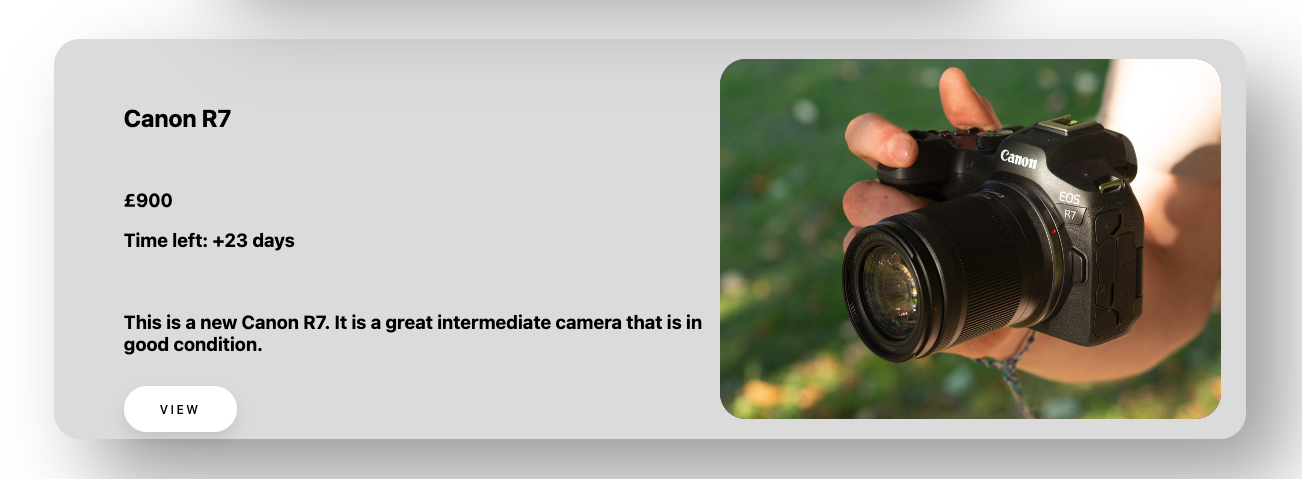
\includegraphics[width=51mm]{ch4_testing_for_eval/media/image28.png} \\ \hline
Search box is displayed on search page & Normal & Search box on page &
Pass -- box displayed &
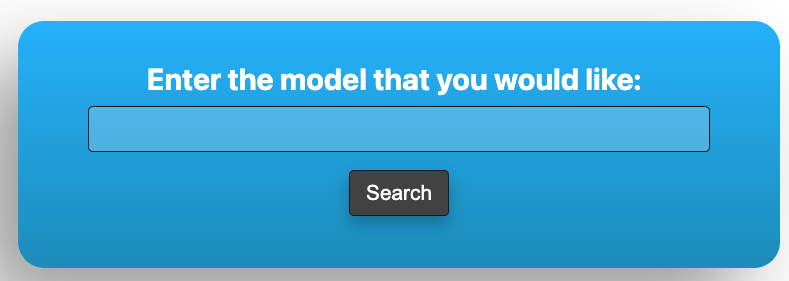
\includegraphics[width=51mm]{ch4_testing_for_eval/media/image29.png} \\ \hline
Search box shows listing from search term & Normal & Listing is
displayed & Pass -- listing found &
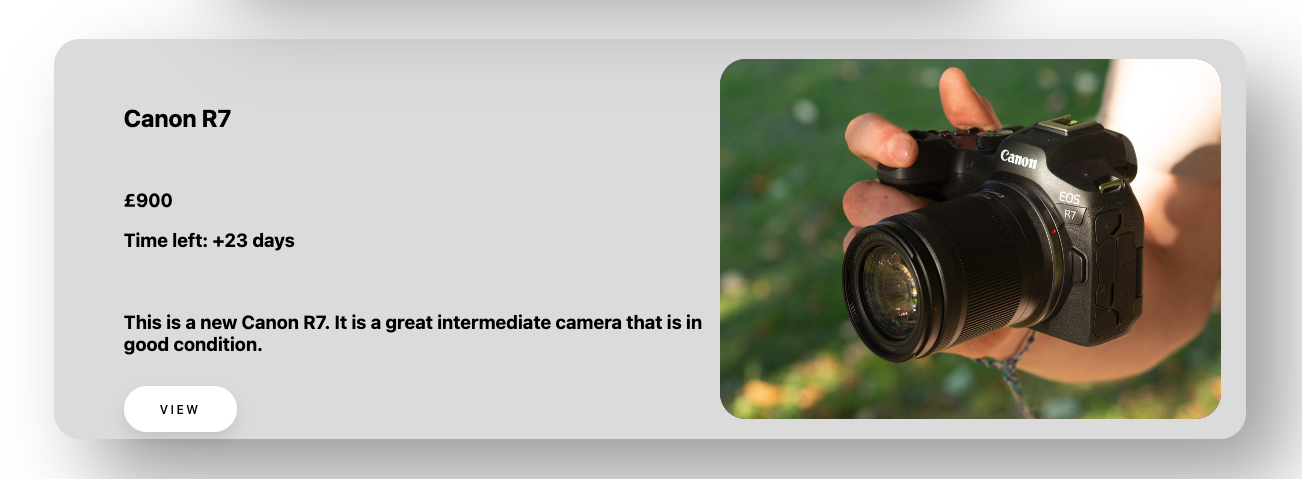
\includegraphics[width=51mm]{ch4_testing_for_eval/media/image28.png} \\ \hline
Search box finds no results & Normal & No results found message & Pass
-- as expected &

\includegraphics[width=51mm]{ch4_testing_for_eval/media/image30.png} \\ \hline
Search box has long search term & Boundary & Works as normal & Pass --
no change &
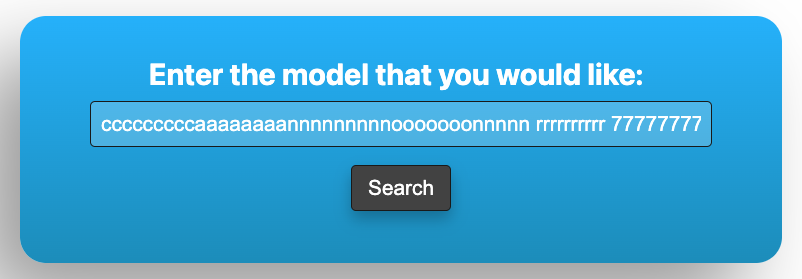
\includegraphics[width=51mm]{ch4_testing_for_eval/media/image31.png}


\includegraphics[width=51mm]{ch4_testing_for_eval/media/image32.png} \\ \hline
View listing button takes user to listing page & Normal & User forwarded
to listings specific page & Pass -- listing is shown &
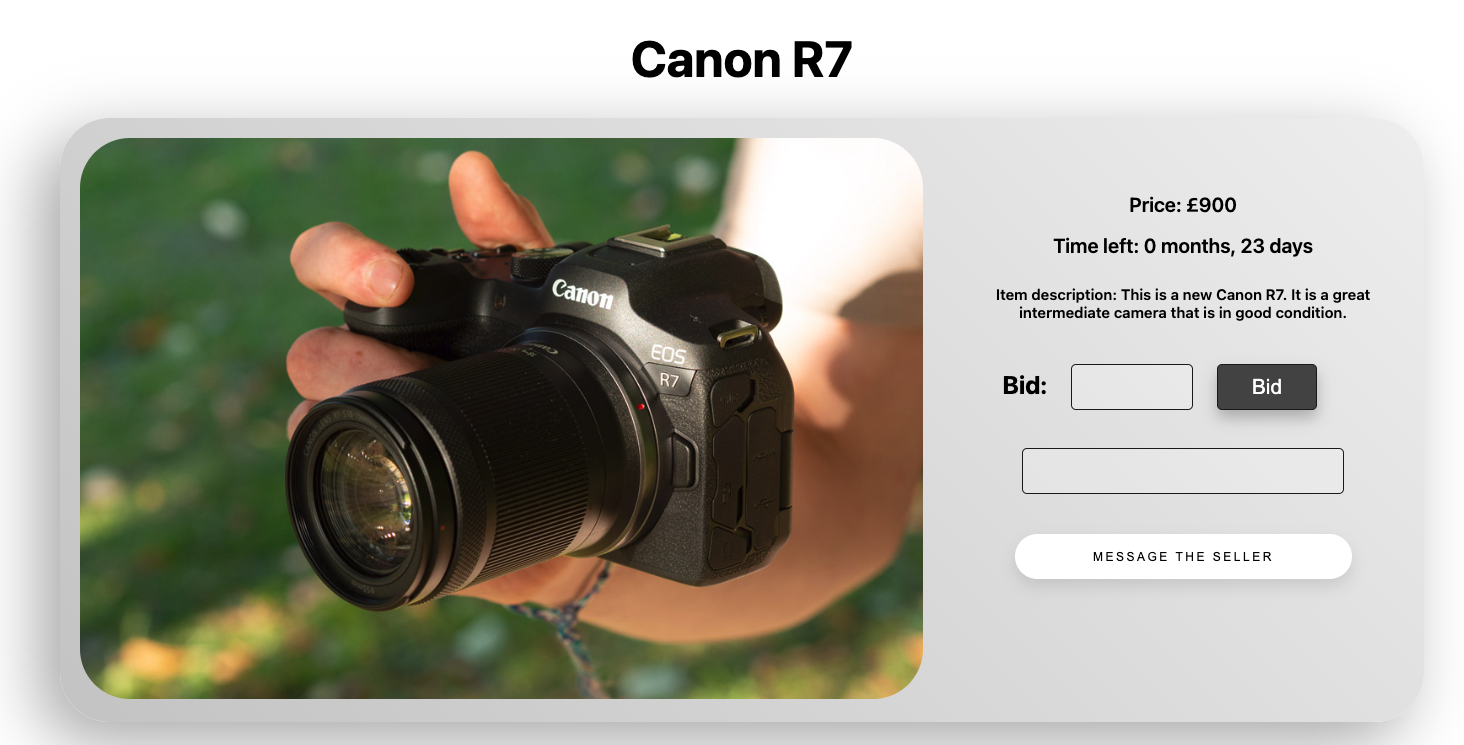
\includegraphics[width=51mm]{ch4_testing_for_eval/media/image33.png} \\ \hline
All listing information is displayed & Normal & All information for a
specific listing is shown & Pass -- all information is shown &
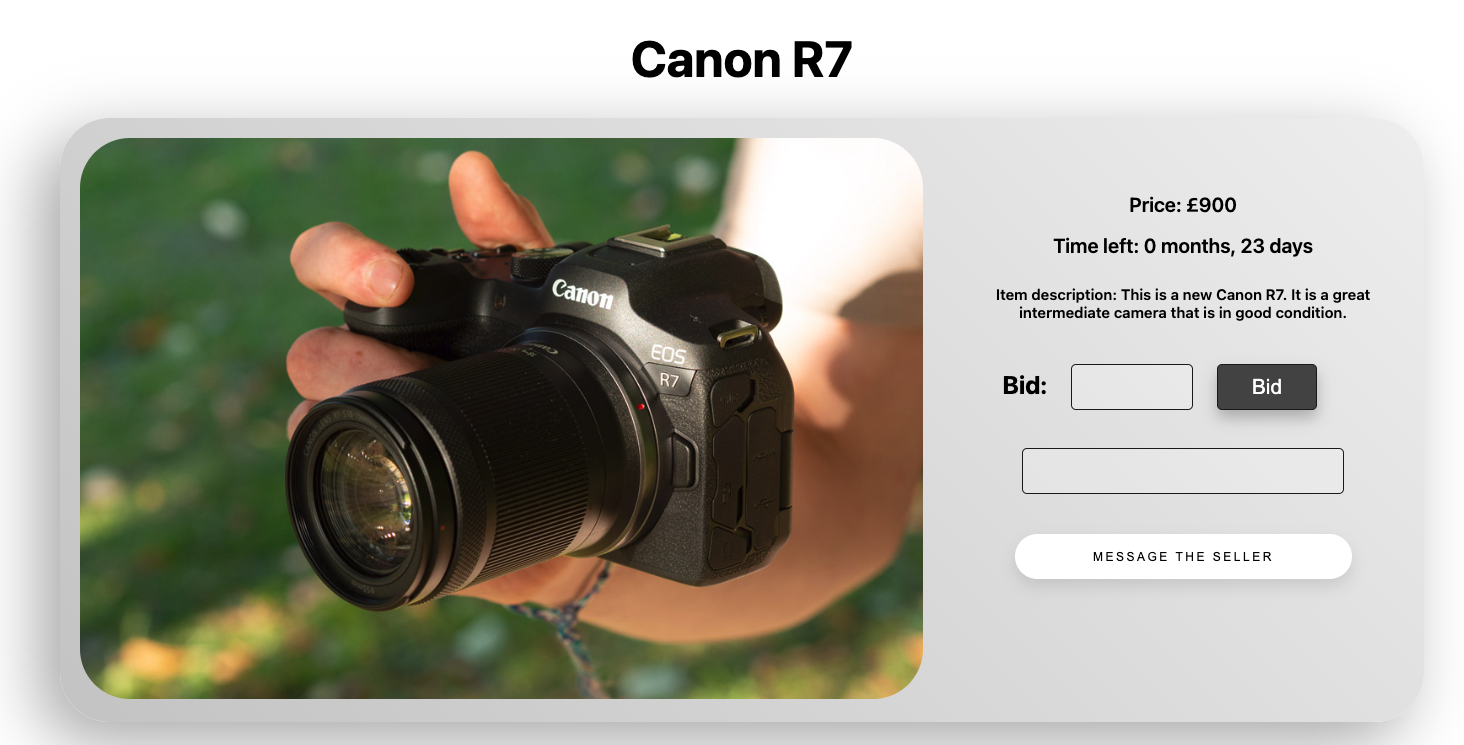
\includegraphics[width=51mm]{ch4_testing_for_eval/media/image33.png} \\ \hline
Bid entered normally & Normal & Bid is processed and updated & Pass --
bid is updated &
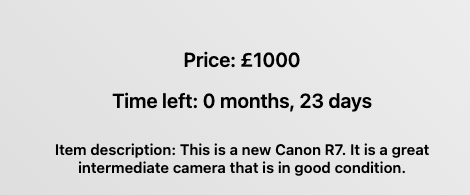
\includegraphics[width=51mm]{ch4_testing_for_eval/media/image34.png} \\ \hline
Bid is not entered & Erroneous & Error is shown & Fail -- no error shown
&
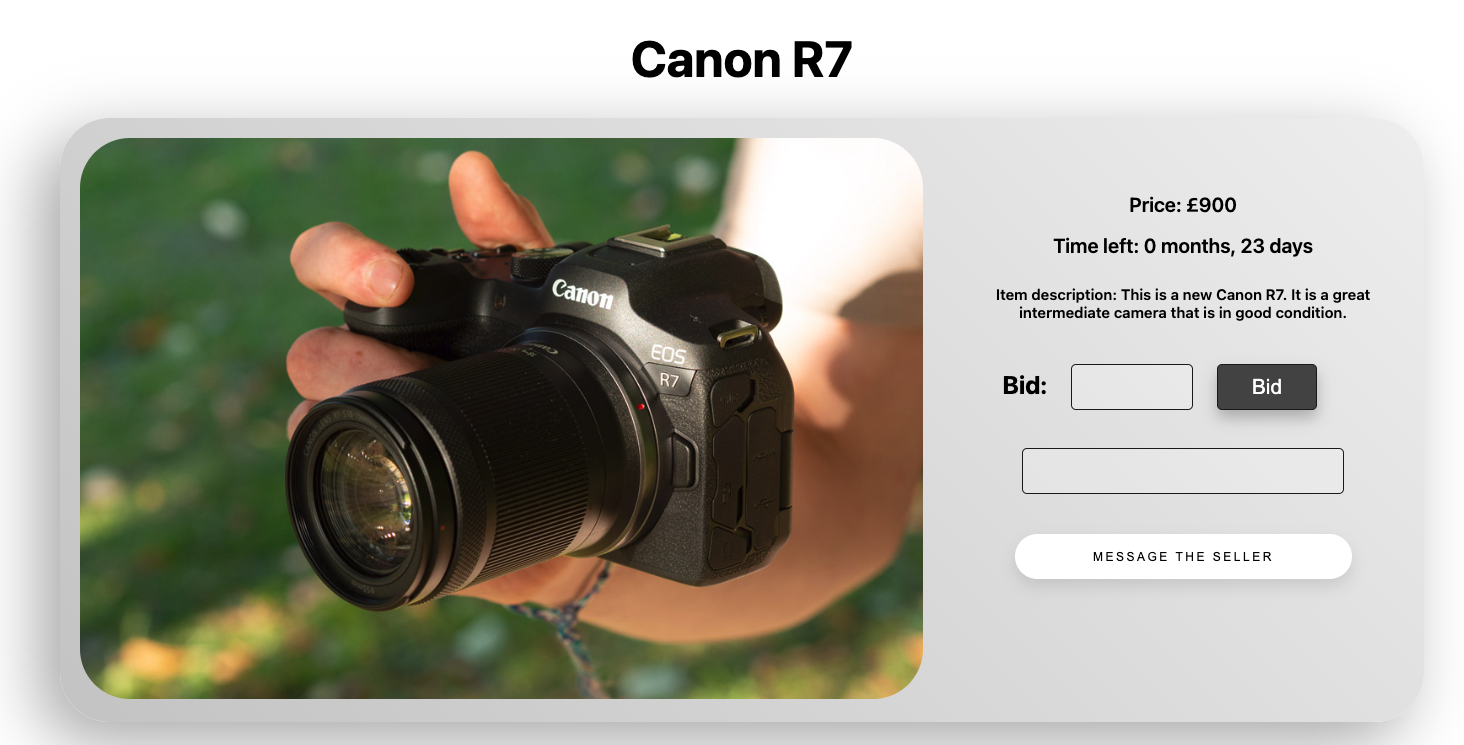
\includegraphics[width=51mm]{ch4_testing_for_eval/media/image33.png} \\ \hline
Bid is not enough & Erroneous & Error is displayed & Pass -- as expected
&
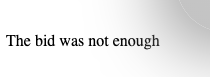
\includegraphics[width=51mm]{ch4_testing_for_eval/media/image35.png} \\ \hline
Large bid entered & Boundary & Function runs normally & Pass -- bid
processed &
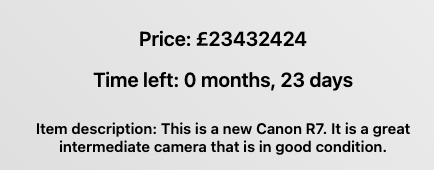
\includegraphics[width=51mm]{ch4_testing_for_eval/media/image36.png} \\ \hline
Message can be entered & Normal & Text can be entered into the message
box & Pass -- as expected &
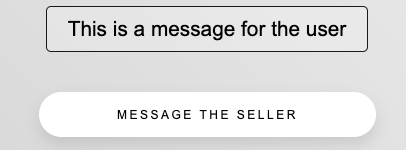
\includegraphics[width=51mm]{ch4_testing_for_eval/media/image37.png} \\ \hline
Message can be sent to seller & Normal & Message processed and then can
be retrieved & Pass -- message shown on messages page &

\includegraphics[width=51mm]{ch4_testing_for_eval/media/image38.png} \\ \hline
No message entered & Erroneous & Error shown to user & Fail -- Message
is processed with empty message shown &
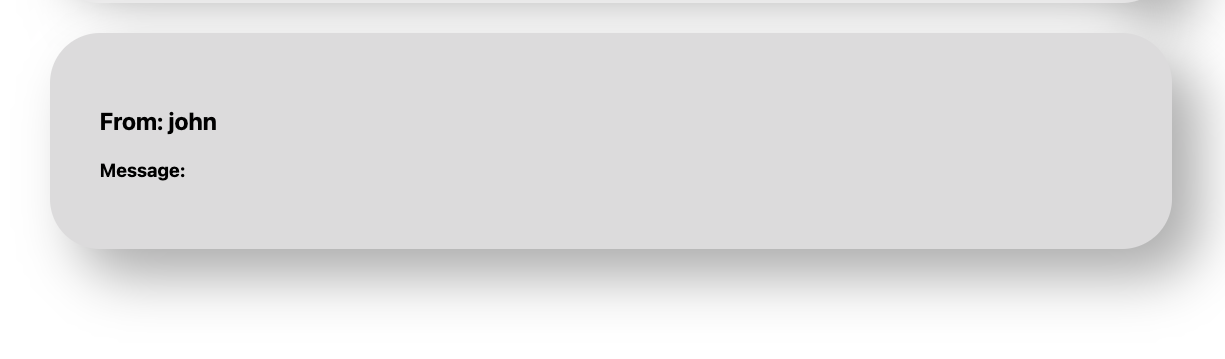
\includegraphics[width=51mm]{ch4_testing_for_eval/media/image39.png} \\ \hline
Messages are retrieved & Normal & Messages are shown when message page
loaded & Pass -- all messages retrieved &
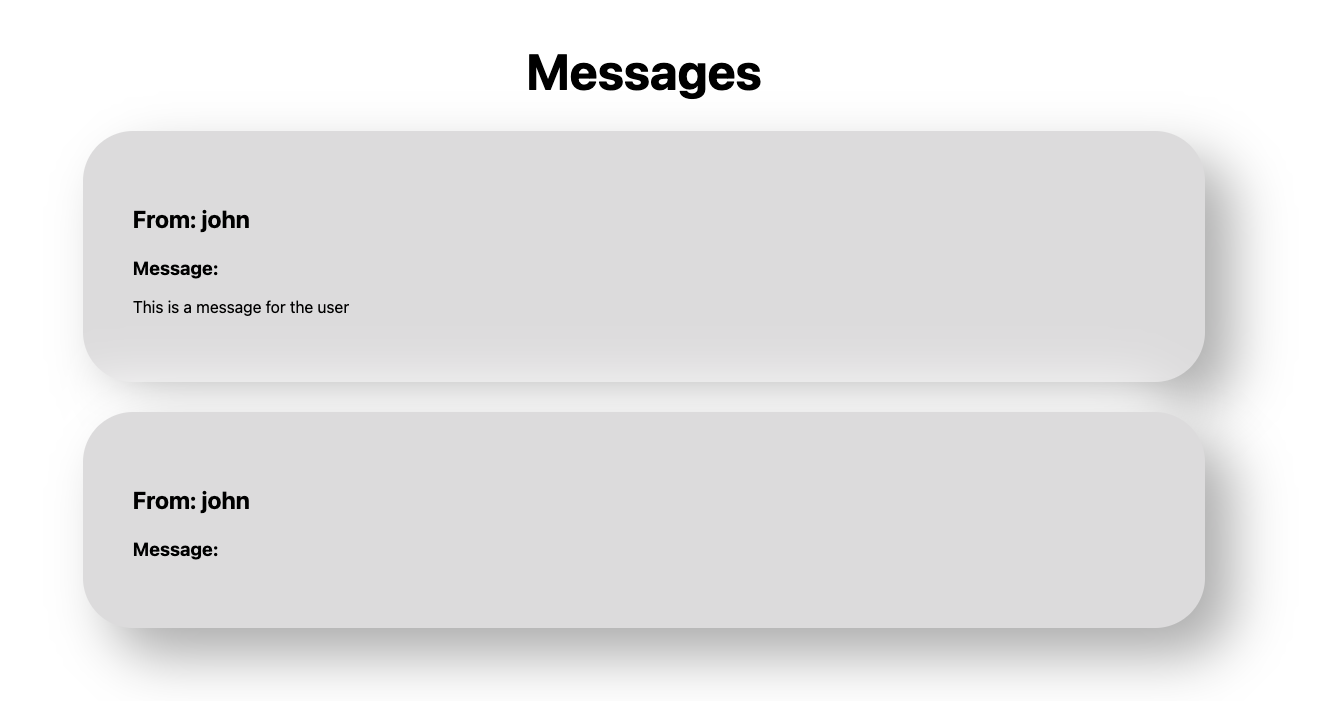
\includegraphics[width=51mm]{ch4_testing_for_eval/media/image40.png} \\ \hline
Price recommendation page shows text box & Normal & Box displayed on the
webpage & Pass -- box shown &
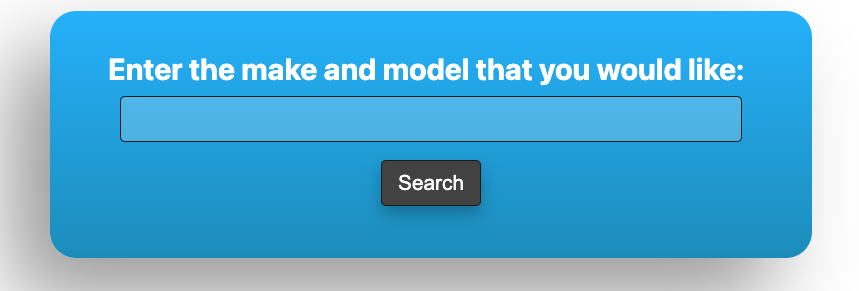
\includegraphics[width=51mm]{ch4_testing_for_eval/media/image41.png} \\ \hline
User can type in price recommendation box & Normal & User is able to
enter text & Pass -- user can type &
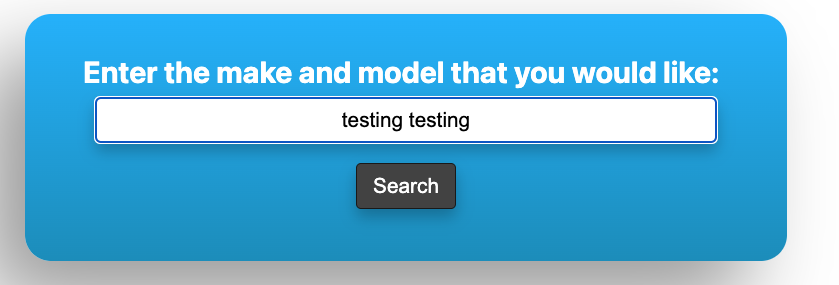
\includegraphics[width=51mm]{ch4_testing_for_eval/media/image42.png} \\ \hline
No text is entered into box & Erroneous & Error is displayed to the user
& Pass -- error displayed &

\includegraphics[width=51mm]{ch4_testing_for_eval/media/image43.png} \\ \hline
Price recommendation is fetched & Normal & Price recommendation is
displayed to the user & Pass -- Information displayed &

\includegraphics[width=51mm]{ch4_testing_for_eval/media/image44.png} \\ \hline
Price recommendation updated on page run & Normal & D3500 price will
change if code is ran & Pass -- price is updated &

\includegraphics[width=51mm]{ch4_testing_for_eval/media/image45.png} \\ \hline
Sign out button & Normal & User is sent back to index page & Pass -- as
expected &
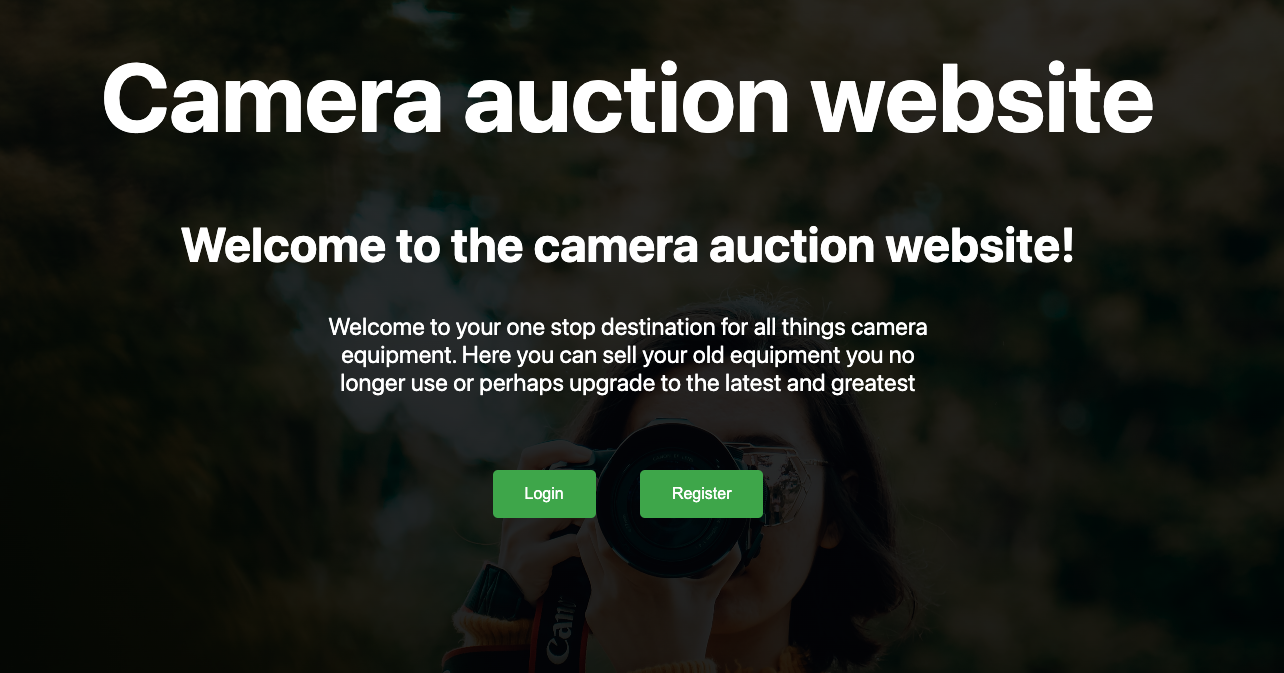
\includegraphics[width=51mm]{ch4_testing_for_eval/media/image46.png} \\ \hline

    \caption{Alpha testing table}
\label{tab:alpha_testing}
\end{longtable}
\end{center}